% Chapter Template

\chapter{Project Planning} % Main chapter title

\label{Chapter3} % Change X to a consecutive number; for referencing this chapter elsewhere, use \ref{ChapterX}

%----------------------------------------------------------------------------------------
%	SECTION 1
%----------------------------------------------------------------------------------------

\section{Tasks description}
\subsection{GEP}
This task corresponds to the work done during the GEP course. This task has not any dependency but the work done will be used for the final documentation.\\

The estimated time for this stage is 70 hours.
\subsection{Initial Stage}
This stage will be used for defining the requisites to accomplish, the architecture of the software and refactor the previous code. Also the required tools will be installed. \\

The estimated time for this stage is 90 hours.
\subsection{Iterations}
Because Agile methodology will be followed, the project has been divided into iterations. There will be a total of 3 iterations: Pseudo-Boolean minimization, Timeout strategies, and multithreading.\\

For each iteration, 80h of work are estimated.
\subsubsection{Planning}
This stage will be used for defining the scope of the iteration and goals.\\

This stage will be 10 hours long.
\subsubsection{Development and TDD}
In this stage the iteration will be developed and tested.\\

This stage will be 60 hours long.
\subsubsection{Finalization}
In this stage all possible bugs will be solved and feedback from the supervisor will be taken.\\

This stage will be 10 hours long.


\subsection{Final Stage}
Here, all the development will be finished and it will be used for finishing all the documentation and prepare the final presentation.\\

This stage will take 50 hours.


%----------------------------------------------------------------------------------------
%	SECTION 2
%----------------------------------------------------------------------------------------

\section{Gantt Diagram}

\begin{figure}[hbtp] 
	\centering
	\makebox[\textwidth]{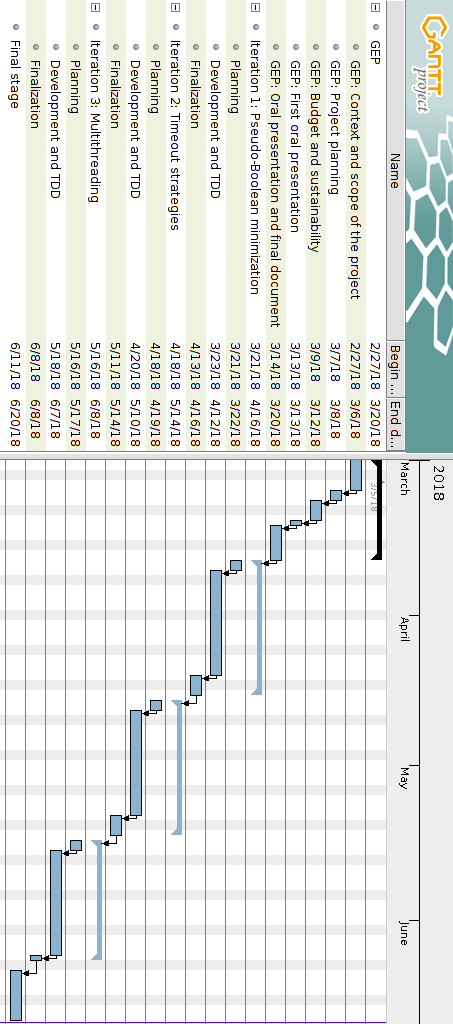
\includegraphics[height=.60\paperheight]{Figures/GanttTable2.png}}
	\caption{Gantt diagram of the project}
	\label{GanttDiagram}
\end{figure}

